\documentclass[10pt,a4paper]{article}
\usepackage[utf8]{inputenc} 
\usepackage[spanish]{babel}
\usepackage{a4wide}
\usepackage{float}
\usepackage{caratula}

\begin{document}

\titulo{Trabajo Práctico}
\subtitulo{SLS: Un simple lenguaje de scripting}

\fecha{\today}

\materia{Teoría de Lenguajes}
\grupo{Los Libres de Contexto}

\integrante{Castro, Alan}{356/10}{alancastro90@gmail.com}
\integrante{Bonomi, Cyntia}{134/03}{cyntiab83@gmail.com}
\integrante{Izcovich, Sabrina}{550/11}{sizcovich@gmail.com}

\maketitle

\tableofcontents

\newpage

\section{Gramática}

En lo que sigue, presentamos la gramática utilizada para la realización del parser:\\

S' $\rightarrow$ program \\ 
program $\rightarrow$ list\_sentencies \\
list\_sentencies $\rightarrow$ NEWLINE a \\
list\_sentencies $\rightarrow$ COMMENT a \\
list\_sentencies $\rightarrow$ sentence a \\
a $\rightarrow$ list\_sentencies \\
a $\rightarrow$ $\lambda$ \\
sentence $\rightarrow$ e SEMICOLON \\
sentence $\rightarrow$ while \\
sentence $\rightarrow$ if\_else \\
sentence $\rightarrow$ for \\
sentence $\rightarrow$ do\_while \\
sentence $\rightarrow$ function SEMICOLON \\
sentence $\rightarrow$ RETURN expression \\
e $\rightarrow$ assignation \\
e $\rightarrow$ advance \\
e $\rightarrow$ ecomparable \\
ecomparable $\rightarrow$ expression \\
ecomparable $\rightarrow$ condition \\
ecomparable $\rightarrow$ conditional \\
possiblecomment $\rightarrow$ COMMENT \\
possiblecomment $\rightarrow$ $\lambda$ \\
comment\_list $\rightarrow$ COMMENT comment\_list \\
comment\_list $\rightarrow$ NEWLINE comment\_list \\
comment\_list $\rightarrow$ $\lambda$ \\
possiblenewline $\rightarrow$ NEWLINE \\
possiblenewline $\rightarrow$ $\lambda$ \\
while $\rightarrow$ WHILE LPAREN condition RPAREN possiblecomment possiblenewline keys \\
if\_else $\rightarrow$ if possibleelse \\
possibleelse $\rightarrow$ ELSE possiblecomment possiblenewline keys \\
if $\rightarrow$ IF LPAREN condition RPAREN possiblecomment possiblenewline keys \\
conditional $\rightarrow$ LPAREN condition RPAREN QUESTIONMARK ecomparable COLON expression \\
possibleelse $\rightarrow$ $\lambda$ \\
conditional $\rightarrow$ condition QUESTIONMARK ecomparable COLON expression \\
for $\rightarrow$ FOR LPAREN assignationorlambda SEMICOLON condition SEMICOLON advancefor RPAREN possiblecomment possiblenewline keys \\
do\_while $\rightarrow$ DO keys\_do WHILE LPAREN condition RPAREN SEMICOLON possiblecomment possiblenewline \\
keys\_do $\rightarrow$ comment\_list sentence possiblenewline \\
keys\_do $\rightarrow$ LKEY possiblenewline possiblecomment list\_sentencies RKEY possiblenewline \\
keys $\rightarrow$ comment\_list sentence possiblenewline \\
keys $\rightarrow$ LKEY possiblenewline possiblecomment list\_sentencies RKEY possiblenewline \\
assignationorlambda $\rightarrow$ assignation \\
assignationorlambda $\rightarrow$ $\lambda$ \\
assignation $\rightarrow$ VAR b \\
b $\rightarrow$ LBRACKET expression RBRACKET ASSIGN expression \\
b $\rightarrow$ ASSIGN ecomparable \\
b $\rightarrow$ COLON ecomparable \\
advancefor $\rightarrow$ advance \\
advancefor $\rightarrow$ assignationorlambda \\
advance $\rightarrow$ VAR c \\
c $\rightarrow$ INCREMENT \\
c $\rightarrow$ PLUSEQUAL value \\
c $\rightarrow$ DECREMENT \\
c $\rightarrow$ MINEQUAL value \\
condition $\rightarrow$ condition OR x \\
condition $\rightarrow$ x \\
x $\rightarrow$ x AND y \\
x $\rightarrow$ y \\
y $\rightarrow$ NOT y \\
y $\rightarrow$ LPAREN condition RPAREN \\
y $\rightarrow$ logical\_condition \\
y $\rightarrow$ value \\
logical\_condition $\rightarrow$ ecomparable i \\
i $\rightarrow$ LESS possibleparen \\
i $\rightarrow$ GREATER possibleparen \\
i $\rightarrow$ EQUAL possibleparen \\
i $\rightarrow$ UNEQUAL possibleparen \\
possibleparen $\rightarrow$ LPAREN ecomparable RPAREN \\
possibleparen $\rightarrow$ ecomparable \\
value $\rightarrow$ STRING \\
value $\rightarrow$ bool \\
value $\rightarrow$ num \\
value $\rightarrow$ function\_with\_return \\
value $\rightarrow$ LBRACKET expression list\_values RBRACKET \\
value $\rightarrow$ LKEY list\_registers RKEY \\
value $\rightarrow$ VAR j \\
j $\rightarrow$ LBRACKET expression RBRACKET \\
j $\rightarrow$ $\lambda$ \\
list\_registers $\rightarrow$ assignation l \\
l $\rightarrow$ COMMA list\_registers \\
list\_values $\rightarrow$ COMMA expression list\_values \\
list\_values $\rightarrow$ $\lambda$ \\
l $\rightarrow$ $\lambda$ \\
expression $\rightarrow$ expression PLUS term \\
expression $\rightarrow$ expression MINUS term \\
expression $\rightarrow$ term \\
term $\rightarrow$ term POW factor \\
term $\rightarrow$ term TIMES factor \\
term $\rightarrow$ term DIVIDE factor \\
term $\rightarrow$ term MODULE factor \\
factor $\rightarrow$ LPAREN expression RPAREN \\
factor $\rightarrow$ value \\
term $\rightarrow$ factor \\
function $\rightarrow$ function\_with\_return \\
function $\rightarrow$ PRINT LPAREN ecomparable RPAREN \\
function\_with\_return $\rightarrow$ MULTIPLICACIONESCALAR LPAREN param\_me RPAREN \\
function\_with\_return $\rightarrow$ CAPITALIZAR LPAREN ecomparable RPAREN \\
function\_with\_return $\rightarrow$ COLINEALES LPAREN VAR COMMA VAR RPAREN \\
function\_with\_return $\rightarrow$ LENGTH LPAREN param\_length RPAREN \\
param\_me $\rightarrow$ VAR COMMA value n \\
n $\rightarrow$ COMMA bool \\
n $\rightarrow$ $\lambda$ \\
param\_length $\rightarrow$ VAR \\
param\_length $\rightarrow$ function\_with\_return \\
param\_length $\rightarrow$ LBRACKET value list\_values RBRACKET \\
param\_length $\rightarrow$ STRING \\
num $\rightarrow$ DECIMAL \\
num $\rightarrow$ NATURAL \\
bool $\rightarrow$ TRUE \\
bool $\rightarrow$ FALSE \\

\newpage
\subsection{Atributos}

Dada la limitación de \textit{PLY} para manejar atributos heredados, todos nuestros atributos son sintetizados.\\

Los atributos con los que contamos son:
\begin{itemize}
\item \textbf{NoTerminal.value}: Consiste en el valor asociado
\item \textbf{NoTerminal.type}: \textit{tipo}. Representa el tipo asociado. El tipo puede ser ``natural'', ``negativo'', ``decimal'' o ``string''.
\item \textbf{NoTerminal.isTrue}: \textit{bool}. Almacena la información del booleano dado por parámetro en multiplicacionEscalar.
\item \textbf{NoTerminal.isArray}: \textit{bool}. Guarda la información de si el no terminal deriva en un arreglo o no.
\end{itemize}

\section{Ejemplo de la Gramática de Atributos}

\begin{figure}[H]
\begin{center}
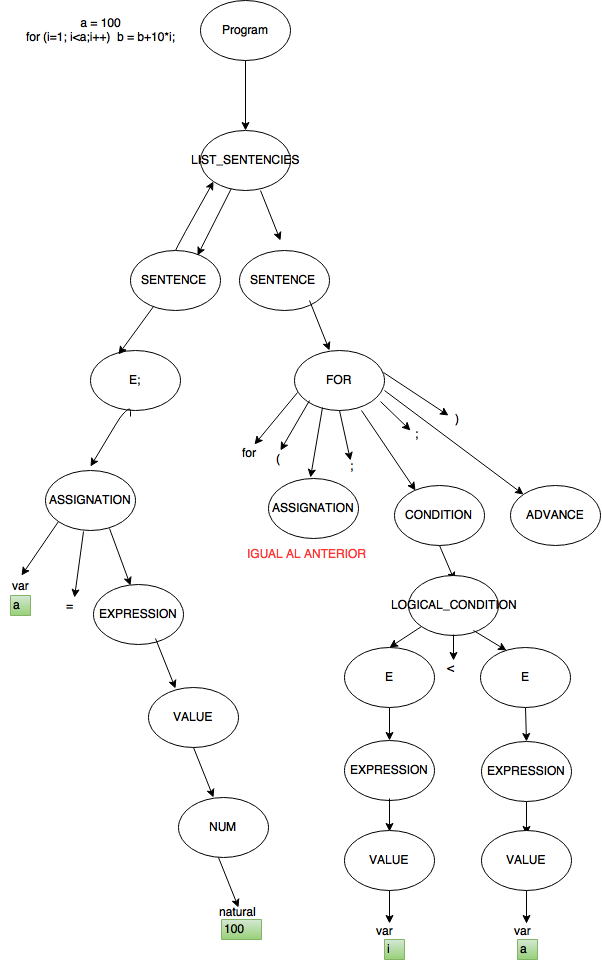
\includegraphics[scale=0.7]{imgs/ejemploGramatica.png}
\end{center}
\end{figure}

En el diagrama anterior, se pueden observar las derivaciones de una parte del programa presentado a modo de ejemplo.

\section{Conflicto}
Nuestro conflicto se presenta en el \textbf{ELSE} en el siguiente caso:

\begin{verbatim}
sentence -> IF LPAREN expression RPAREN keys . possibleelse
possibleelse -> . ELSE keys
possibleelse -> .
\end{verbatim}

Consiste en un conflicto de tipo shift/reduce dado que el parser no sabe si debe seguir avanzando por el else o reducir lo anterior. Para resolverlo, habría que reescribir todas las reglas para el else.

\section{Descripción}

Dadas las decisiones tomadas al momento de formular la gramática, consideramos los siguientes casos como incorrectos:

\begin{itemize}
\item Asumimos que los Registers toman únicamente literales de tipos básicos.
\item En el caso de la operación potencia, nos basamos en la documentación de C++ para definir el tipo asignado. Dado que en todos los casos el resultado es de tipo punto flotante\footnote{http://en.cppreference.com/w/cpp/numeric/math/pow}, decidimos mantenerlo, por lo que la indexación con una potencia genera un error de tipos. Por ejemplo, g[b ^ b] falla.
\end{itemize}

Para el resguardo de las variables con sus atributos utilizamos un diccionario \textit{table} donde se almacena la información: \textbf{nombre, tipo, isArray, isTrue} para las variables que así lo requieran para la ejecución de funciones que las utilizan.

\section{Compilación y ejecución}
Para compilar nuestro trabajo práctico y ejecutarlo, alcanza con correr en la consola el siguiente comando:
\textbf{./SLSparser.py -o archivoSalida -c archivoEntrada} 
Los parámetros son opcionales. Por default, la entrada y salida son la consola en el caso en el que no se especifique alguno de los archivos.
Al pasar un programa por stdin, la finalización del mismo se indica a través del comando \textit{ctrl+d}

\section{Casos de prueba}
Los casos de prueba utilizados fueron los del enunciado, con los que nos aseguramos que se devolviera un error en cuanto la sintáxis no era correcta. Dadas algunas decisiones mencionadas anteriormente, no todos los tests de la cátedra son aceptados por nuestra gramática. En particular, agregamos la carpeta \textbf{test} con los casos de tests subidos por la cátedra con algunas modificaciones para los casos que excluímos.

\section{Conclusión}
Podemos concluir que resulta muy complicado realizar una gramática de tal dimensión sin tener problemas de ambigüedad. A pesar de ello, PLY es una excelente herramienta para dicho fin dado que resuelve los conflictos solucionándole muchos problemas al programador.

\section{Referencias}
\begin{itemize}
\item \textbf{Aho, Sethi, Ullman}, \textit{Compilers: Principles, Techniques, and Tools}, Addison-Wesley, 1986. ISBN 0-201-10088-6

\item \textbf{Python Lex-Yacc} \textit{http://www.dabeaz.com/ply/}
\end{itemize}

\end{document}
